\chapter{Performance Analysis}

\section{Theoretical Performance Analysis}

\subsection{Computational Cost}

Computational cost directly determines how efficiently an authentication scheme
can be deployed on resource-constrained hardware.
The Python cryptographic library \texttt{pycrypto} is used in a Windows environment
to measure the computational cost of core cryptographic functions, such as SHA-256
($T_{\mathsf{hash}}$), AES Encryption/Decryption ($T_{\mathsf{aes}}$), and random
generation ($T_{\mathsf{rand}}$).
The PUF operation cost ($T_{\mathsf{puf}}$) is taken from prior benchmarks on the
same platform~\cite{zheng2022puf}.
Benchmark averages over 100 iterations are: $T_{\mathsf{rand}} = 0.0018$\,ms,
$T_{\mathsf{puf}} = 0.0522$\,ms, $T_{\mathsf{hash}} = 0.0353$\,ms,
$T_{\mathsf{aes}} = 0.0867$\,ms.

\subsubsection{Enrolment Phase}

To execute the node enrolment phase:
\begin{itemize}
  \item $AS$ computes two random generations ($T_{\mathsf{rand}}$), one PUF
    operation ($T_{\mathsf{puf}}$), and two hash operations ($T_{\mathsf{hash}}$)
    for pseudonym initialisation.
  \item $D$ executes two random generations ($T_{\mathsf{rand}}$) and one PUF
    operation ($T_{\mathsf{puf}}$).
\end{itemize}

Hence, the total computational cost per node enrolment amounts to
$2T_{\mathsf{puf}} + 2T_{\mathsf{hash}} + 4T_{\mathsf{rand}} = \mathbf{0.18}$\,ms.
The proposed scheme incurs a marginal overhead of 0.03\,ms over DAuth~\cite{das2026comsnets}
(0.15\,ms), directly attributable to the additional hash operation for pseudonym
initialisation, a security feature absent from DAuth.
Table~\ref{tab:comp_enroll} compares the enrolment computational cost.

\begin{table}[!ht]
  \centering
  \caption{Computational Cost Comparison: Enrolment Phase.}
  \label{tab:comp_enroll}
  \small
  \setlength{\tabcolsep}{5pt}
  \begin{tabular}{lll}
    \toprule
    Scheme & Operations & Cost (ms) \\
    \midrule
    LAAKA~\cite{ali2024laaka}          & $3T_\mathsf{hash}$ & 0.11 \\
    Zhou~\cite{zhou2024auth}           & $T_\mathsf{puf}+2T_\mathsf{hash}+3T_\mathsf{rand}$ & 0.13 \\
    Zheng et al.~\cite{zheng2022puf}   & $2T_\mathsf{puf}+8T_\mathsf{hash}+4T_\mathsf{aes}+5T_\mathsf{rand}$ & 0.69 \\
    He et al.~\cite{he2023lightweight} & $4T_\mathsf{hash}+T_\mathsf{aes}+T_\mathsf{rand}$ & 0.23 \\
    DAuth~\cite{das2026comsnets}        & $2T_\mathsf{puf}+1T_\mathsf{hash}+4T_\mathsf{rand}$ & 0.15 \\
    \textbf{Proposed}                  & $2T_\mathsf{puf}+2T_\mathsf{hash}+4T_\mathsf{rand}$ & \textbf{0.18} \\
    \bottomrule
  \end{tabular}\\[4pt]
  \small Benchmark (avg.\ 100 iterations): $T_\mathsf{rand}$=0.0018\,ms,
  $T_\mathsf{puf}$=0.0522\,ms, $T_\mathsf{hash}$=0.0353\,ms, $T_\mathsf{aes}$=0.0867\,ms.
\end{table}

\subsubsection{Authentication and Key Exchange Phase}

In the proposed scheme, $D$ and $AS$ both execute one PUF operation
($T_{\mathsf{puf}}$).
\begin{itemize}
  \item $D$ additionally performs six hash operations ($T_{\mathsf{hash}}$):
    pseudonym computation, unique secret hash, and XOR mask in the Authentication
    Phase, followed by mask recovery, session key derivation, and pseudonym
    rotation in the Key Exchange Phase.
  \item $AS$ performs five hash operations ($T_{\mathsf{hash}}$), along with one
    AES encryption ($T_{\mathsf{aes}}$) for the gateway token and one random
    generation ($T_{\mathsf{rand}}$) for $m_{\mathrm{new}}$.
  \item $GW$ runs one AES decryption ($T_{\mathsf{aes}}$) to recover the session
    key and updated pseudonym from the forwarded token.
\end{itemize}

This leads to a total cost of
$2T_{\mathsf{puf}} + 11T_{\mathsf{hash}} + 2T_{\mathsf{aes}} + T_{\mathsf{rand}}
= \mathbf{0.67}$\,ms.
The proposed scheme incurs a modest overhead of 0.11\,ms over DAuth~\cite{das2026comsnets}
(0.56\,ms), attributable to three additional hash operations for pseudonym computation,
dual-state lookup, and pseudonym rotation, which is the price paid for anonymity and
desynchronisation resilience.
Table~\ref{tab:comp_auth} compares the authentication and key exchange computational
cost.

\begin{table}[!ht]
  \centering
  \caption{Computational Cost Comparison: Authentication \& Key Exchange Phase.}
  \label{tab:comp_auth}
  \small
  \setlength{\tabcolsep}{5pt}
  \begin{tabular}{lll}
    \toprule
    Scheme & Operations & Cost (ms) \\
    \midrule
    LAAKA~\cite{ali2024laaka}          & $16T_\mathsf{hash}$ & 0.56 \\
    Zhou~\cite{zhou2024auth}           & $15T_\mathsf{hash}$ & 0.53 \\
    Zheng et al.~\cite{zheng2022puf}   & $2T_\mathsf{puf}+6T_\mathsf{hash}+4T_\mathsf{aes}+5T_\mathsf{rand}$ & 0.67 \\
    He et al.~\cite{he2023lightweight} & $11T_\mathsf{hash}+5T_\mathsf{aes}+2T_\mathsf{ecc}$ & 1.74 \\
    DAuth~\cite{das2026comsnets}        & $2T_\mathsf{puf}+8T_\mathsf{hash}+2T_\mathsf{aes}+T_\mathsf{rand}$ & 0.56 \\
    \textbf{Proposed}                  & $2T_\mathsf{puf}+11T_\mathsf{hash}+2T_\mathsf{aes}+T_\mathsf{rand}$ & \textbf{0.67} \\
    \bottomrule
  \end{tabular}\\[4pt]
  \small Benchmark (avg.\ 100 iterations): $T_\mathsf{rand}$=0.0018\,ms,
  $T_\mathsf{puf}$=0.0522\,ms, $T_\mathsf{hash}$=0.0353\,ms, $T_\mathsf{aes}$=0.0867\,ms;
  $T_\mathsf{ecc}$=0.461\,ms (scaled from He et al.~\cite{he2023lightweight} hardware ratios).
\end{table}

\subsection{Communication Cost}

Communication cost is a core feature for analysing the performance of an
authentication scheme, based on the number of message exchanges and their sizes (in
bits).
It is assumed that identities and timestamps are 32\,bits, along with nonces, hashes,
challenges, responses, and ciphertexts as 256\,bits, ensuring a fair comparison.

\subsubsection{Enrolment Phase}

During the node enrolment phase, $D$ enrols itself with $AS$, executing three message
exchanges: (1)~$ID_D$ (32\,b) from $D$ to $AS$; (2)~$c_D$ (256\,b) and $m_D$
(256\,b) from $AS$ to $D$; (3)~$y_D$ (256\,b), $R_D$ (256\,b), and $c_{AS\text{-}D}$
(256\,b) from $D$ to $AS$.
Total enrolment communication cost: \textbf{1312\,bits}.
Table~\ref{tab:comm_enroll} shows the comparison.

\begin{table}[!ht]
  \centering
  \caption{Communication Cost Comparison: Enrolment Phase.}
  \label{tab:comm_enroll}
  \small
  \setlength{\tabcolsep}{6pt}
  \begin{tabular}{lcc}
    \toprule
    Scheme & \# Messages & Cost (bits) \\
    \midrule
    LAAKA~\cite{ali2024laaka}          & 3 & 2592 \\
    Zhou~\cite{zhou2024auth}           & 5 & 1344 \\
    Zheng et al.~\cite{zheng2022puf}   & 3 & 1600 \\
    He et al.~\cite{he2023lightweight} & 2 & 1280 \\
    DAuth~\cite{das2026comsnets}        & 3 & 1312 \\
    \textbf{Proposed}                  & 3 & \textbf{1312} \\
    \bottomrule
  \end{tabular}\\[4pt]
  \small IDs/timestamps = 32\,b; hashes/nonces/challenges/ciphertexts = 256\,b.
\end{table}

\subsubsection{Authentication and Key Exchange Phase}

The authentication and key exchange phase is executed using three message
communications.
Message 1 ($D \to AS$): $\mathit{PID}$ (256\,b) + $Y_{AS\text{-}D}^H$ (256\,b) +
$ts_1$ (32\,b).
Message 2 ($AS \to D$): $m_H$ (256\,b) + $ts_2$ (32\,b).
Message 3 ($AS \to GW$): $\mathit{PID}_{\mathrm{new}}$ (256\,b) + $ID_{AS}$ (32\,b)
+ $\mathsf{auth\_token}_D$ (256\,b).
Total: \textbf{1376\,bits}.
Table~\ref{tab:comm_auth} shows the comparison.

\begin{table}[!ht]
  \centering
  \caption{Communication Cost Comparison: Authentication \& Key Exchange Phase.}
  \label{tab:comm_auth}
  \small
  \setlength{\tabcolsep}{6pt}
  \begin{tabular}{lcc}
    \toprule
    Scheme & \# Messages & Cost (bits) \\
    \midrule
    LAAKA~\cite{ali2024laaka}          & 3 & 2400 \\
    Zhou~\cite{zhou2024auth}           & 4 & 2464 \\
    Zheng et al.~\cite{zheng2022puf}   & 3 & 1600 \\
    He et al.~\cite{he2023lightweight} & 3 & 1120 \\
    DAuth~\cite{das2026comsnets}        & 3 & 928 \\
    \textbf{Proposed}                  & 3 & \textbf{1376} \\
    \bottomrule
  \end{tabular}\\[4pt]
  \small IDs/timestamps = 32\,b; hashes/nonces/challenges/ciphertexts = 256\,b.
\end{table}

DAuth~\cite{das2026comsnets} requires 928\,bits; the 448-bit increase in the proposed
scheme directly reflects the widening of the device identifier from a 32-bit $ID_D$
to a 256-bit pseudonym $\mathit{PID}$, which is the direct cost of adding device
anonymity to all open-channel communications.
The proposed scheme matches DAuth exactly in the enrolment phase (1312\,bits),
demonstrating that pseudonym initialisation adds no communication overhead over the
DAuth at registration.

\FloatBarrier
\section{Simulation-Based Performance Analysis}
\label{sec:sim}

A simulation-based performance evaluation has been conducted using the COOJA
simulator within the Contiki-NG framework.
Three complementary studies are reported.
\begin{enumerate}
  \item \textbf{Overall per-device comparison:} Proposed scheme vs.\
    DAuth~\cite{das2026comsnets}, LAAKA~\cite{ali2024laaka}, and Zhou~\cite{zhou2024auth}
    in a fixed 100-node network (1 GW, 79 AS nodes with 2 active, 20 newly joined devices).
  \item \textbf{AS pool-size study:} Active AS nodes varied from 2 to 10.
  \item \textbf{Network scalability study:} Network size $N$ varied across
    $\{30, 50, 80, 100, 120\}$ nodes, with 20\,\% of nodes as newly joined devices.
\end{enumerate}
All results are averaged over ten independent random seeds.
Table~\ref{tab:simparams} lists the common simulation parameters.

\begin{table}[!ht]
  \centering
  \caption{Simulation Parameters.}
  \label{tab:simparams}
  \small
  \setlength{\tabcolsep}{5pt}
  \begin{tabular}{ll}
    \toprule
    Parameter & Value \\
    \midrule
    Operating System     & Contiki-NG \\
    Mote Type            & Cooja Mote \\
    Network Size         & 100 Nodes \\
    Propagation Model    & UDGM (Distance Loss) \\
    Application Layer    & CoAP \\
    Network Layer        & RPL Lite \\
    MAC Layer            & CSMA / IEEE 802.15.4 \\
    Simulation Time      & 75 Seconds \\
    No.\ of Simulations  & 10 per configuration \\
    Schemes compared     & Proposed, DAuth~\cite{das2026comsnets}, LAAKA~\cite{ali2024laaka}, Zhou~\cite{zhou2024auth} \\
    Active AS (study ii) & 2, 5, 10 \\
    Network size (study iii) & $N \in \{30, 50, 80, 100, 120\}$ \\
    \bottomrule
  \end{tabular}
\end{table}

\subsection{Overall Per-Device Cost}

For 20 newly joined nodes in a fixed 100-node network with two active authentication
servers, the proposed scheme demonstrated a consistent advantage over LAAKA and Zhou.
As shown in Figure~\ref{fig:sim_total}(a), the proposed scheme achieves a reduction
of \textbf{42.8\,\%} and \textbf{32.4\,\%} in per-device energy consumption
over LAAKA and Zhou et al., respectively.
Similarly, a reduction of \textbf{42.8\,\%} and \textbf{32.4\,\%} is demonstrated
in per-device CPU time (Figure~\ref{fig:sim_total}(b)).
DAuth~\cite{das2026comsnets} sits just below the proposed scheme in both metrics,
as it requires no pseudonym operations; the proposed scheme pays a small overhead
(approximately 8\,\%) for the pseudonym-rotation and dual-state mechanisms that
deliver anonymity and desynchronisation resilience, both of which are absent from DAuth.
Due to the incorporation of fewer message exchanges and lightweight
hash-XOR operations, the proposed scheme minimises radio activity---the dominant
energy cost in multihop IoT---compared to the more message-intensive
LAAKA and Zhou et al.\ schemes.

\begin{figure}[!ht]
  \centering
  
\includegraphics[width=0.92\textwidth]{fig_sim_total}
  \caption{Per-device mean total cost, all phases:
           (a)~energy and (b)~CPU time, 100-node network, 10 seeds.}
  \label{fig:sim_total}
\end{figure}

\subsection{Authentication Server Pool Size}

In the decoupled design, the gateway selects any capable node as the authentication
server, so the size of the AS pool directly influences load distribution and overall
network performance.
The performance of the proposed scheme, DAuth, LAAKA, and Zhou is evaluated by
varying the number of active AS nodes from 2 to 10.

Considering the total energy consumption (Figure~\ref{fig:sim_as}(a)), a reduction
of approximately \textbf{42\,\%} is demonstrated by the proposed scheme over LAAKA
at every AS count.
Both the proposed scheme and DAuth improve as the pool grows from 2 to 10 servers,
since additional authenticators absorb the join load of newly arrived devices.
As shown in Figure~\ref{fig:sim_as}(b), a reduction of approximately 42\,\% in
total CPU time is demonstrated over LAAKA across all AS counts.
Zhou et al.\ shows essentially flat cost across all AS pool sizes.
DAuth sits consistently just below the proposed scheme, reflecting the absence of
pseudonym-rotation overhead.

\begin{figure}[!ht]
  \centering
  \begin{subfigure}[b]{0.72\linewidth}
    
\includegraphics[width=\linewidth]{fig_sim_as_energy}
    \caption{Total energy vs.\ number of active AS nodes.}
  \end{subfigure}
  \par\vspace{8pt}
  \begin{subfigure}[b]{0.72\linewidth}
    
\includegraphics[width=\linewidth]{fig_sim_as_cpu}
    \caption{Total CPU time vs.\ number of active AS nodes.}
  \end{subfigure}
  \caption{Authentication cost vs.\ AS pool size (20 devices, 5 seeds).}
  \label{fig:sim_as}
\end{figure}

\subsection{Network Scalability}

The performance of authentication schemes is also analysed by considering their
scalability with respect to total network size $N$, varied from 30 to 120 nodes,
where 20\,\% of nodes in each network are newly joined devices.
Considering the total energy consumption (Figure~\ref{fig:sim_network}(a)), at
$N = 120$ the proposed scheme demonstrates a reduction of \textbf{42.7\,\%} over
LAAKA and \textbf{37.6\,\%} over Zhou et al.
Similarly, as shown in Figure~\ref{fig:sim_network}(b), a reduction of 42.7\,\% and
37.6\,\% is demonstrated with respect to total CPU time over LAAKA and Zhou et al.,
respectively, at $N = 120$.
LAAKA and Zhou et al.\ exhibit steeper energy and CPU growth with increasing $N$
because their larger per-device message payloads and additional exchanges accumulate
faster as the device count grows.
DAuth and the proposed scheme both scale favourably, maintaining the lowest total
cost across all network sizes; the proposed scheme incurs only a modest overhead
above DAuth attributable to the additional pseudonym-rotation mechanism.

\begin{figure}[!ht]
  \centering
  \begin{subfigure}[b]{0.72\linewidth}
    
\includegraphics[width=\linewidth]{fig_sim_net_energy}
    \caption{Total energy vs.\ network size $N$.}
  \end{subfigure}
  \par\vspace{8pt}
  \begin{subfigure}[b]{0.72\linewidth}
    
\includegraphics[width=\linewidth]{fig_sim_net_cpu}
    \caption{Total CPU time vs.\ network size $N$.}
  \end{subfigure}
  \caption{Network scalability: total energy and CPU time vs.\ $N$.}
  \label{fig:sim_network}
\end{figure}

\subsection{Desynchronisation Recovery}
\label{sec:desync_perf}

During the Key Exchange Phase, the AS simultaneously dispatches two packets: one to
the gateway carrying $(\mathit{PID}_{\mathrm{new}}, ID_{AS},
\mathsf{auth\_token}_D)$, and one to the device carrying $(m_H, ts_2)$.
Desynchronisation arises when the packet destined for the device is lost in transit.

DAuth~\cite{das2026comsnets} stores only a single nonce state at the AS.
When the device re-authenticates using the old $m_{\mathrm{curr}}$, the AS has no
means to recognise it and rejects the request.
The device must therefore undergo a full re-enrolment before a new authentication
and key exchange can succeed.
The proposed scheme eliminates this penalty through its dual-state mechanism.

Since the dual-state desynchronisation recovery mechanism is a direct extension of
DAuth's single-state protocol, only DAuth serves as the meaningful baseline for this
comparison.

Figure~\ref{fig:desync_bar} presents a per-device energy and CPU time comparison
of a single authentication round under two conditions: normal operation (before any
packet loss) and recovery (the round immediately following a desynchronisation
event), evaluated over a 100-node multi-hop RPL network, 20 devices, and 5 seeds.
As shown in Figure~\ref{fig:desync_bar}(a), DAuth~\cite{das2026comsnets} incurs
134.8\,mJ per recovery round, a 118.3\,\% increase over its normal round cost of
61.8\,mJ, reflecting the overhead of a failed authentication attempt followed by
full re-enrolment.
The proposed scheme's recovery round costs 87.2\,mJ, statistically indistinguishable
from its normal round (98.6\,mJ), confirming that the dual-state mechanism incurs
zero additional overhead during recovery.
Compared directly, the proposed scheme reduces per-device recovery energy by
\textbf{47.6\,mJ (35.3\,\%)} over DAuth~\cite{das2026comsnets}.
The CPU time results in Figure~\ref{fig:desync_bar}(b) exhibit the same pattern:
DAuth~\cite{das2026comsnets} incurs 2.185\,s per recovery round against 1.413\,s for
the proposed scheme, yielding a \textbf{35.3\,\% reduction} in execution time.

\begin{figure}[!ht]
  \centering
  
\includegraphics[width=0.95\textwidth]{fig_desync_bar}
  \caption{Per-device desynchronisation recovery cost: (a)~energy and
           (b)~CPU time for a normal round vs.\ a recovery round, averaged over
           20 devices and 5 seeds in a 100-node RPL network.}
  \label{fig:desync_bar}
\end{figure}

\FloatBarrier
\section{Hardware-Based Performance Analysis}

Hardware-based evaluation validates the feasibility of the proposed scheme by
measuring its performance on physical devices under real operating conditions.

All four schemes (the proposed scheme, DAuth~\cite{das2026comsnets},
LAAKA~\cite{ali2024laaka}, and Zhou et al.~\cite{zhou2024auth}) are implemented on a
\textbf{Raspberry Pi~4B} platform, equipped with a quad-core 64-bit ARM Cortex-A72
processor operating at 1.5\,GHz.
Identical hardware is used across all four schemes to ensure a fair comparison of
energy consumption and CPU time.
The implementation considers two Raspberry Pi~4B platforms as IoT nodes: one
performing the role of the newly joined device, and the other functioning as the
authentication server.
A Windows laptop is leveraged as the gateway.
Each of the three entities maintains direct TCP communication with the others.
Energy consumption is estimated using the active power profile of the Raspberry
Pi~4B (3.8\,W) multiplied by the measured wall-clock time per authentication round.
The physical testbed is shown in Figure~\ref{fig:hw_setup}.

\begin{figure}[!ht]
  \centering
  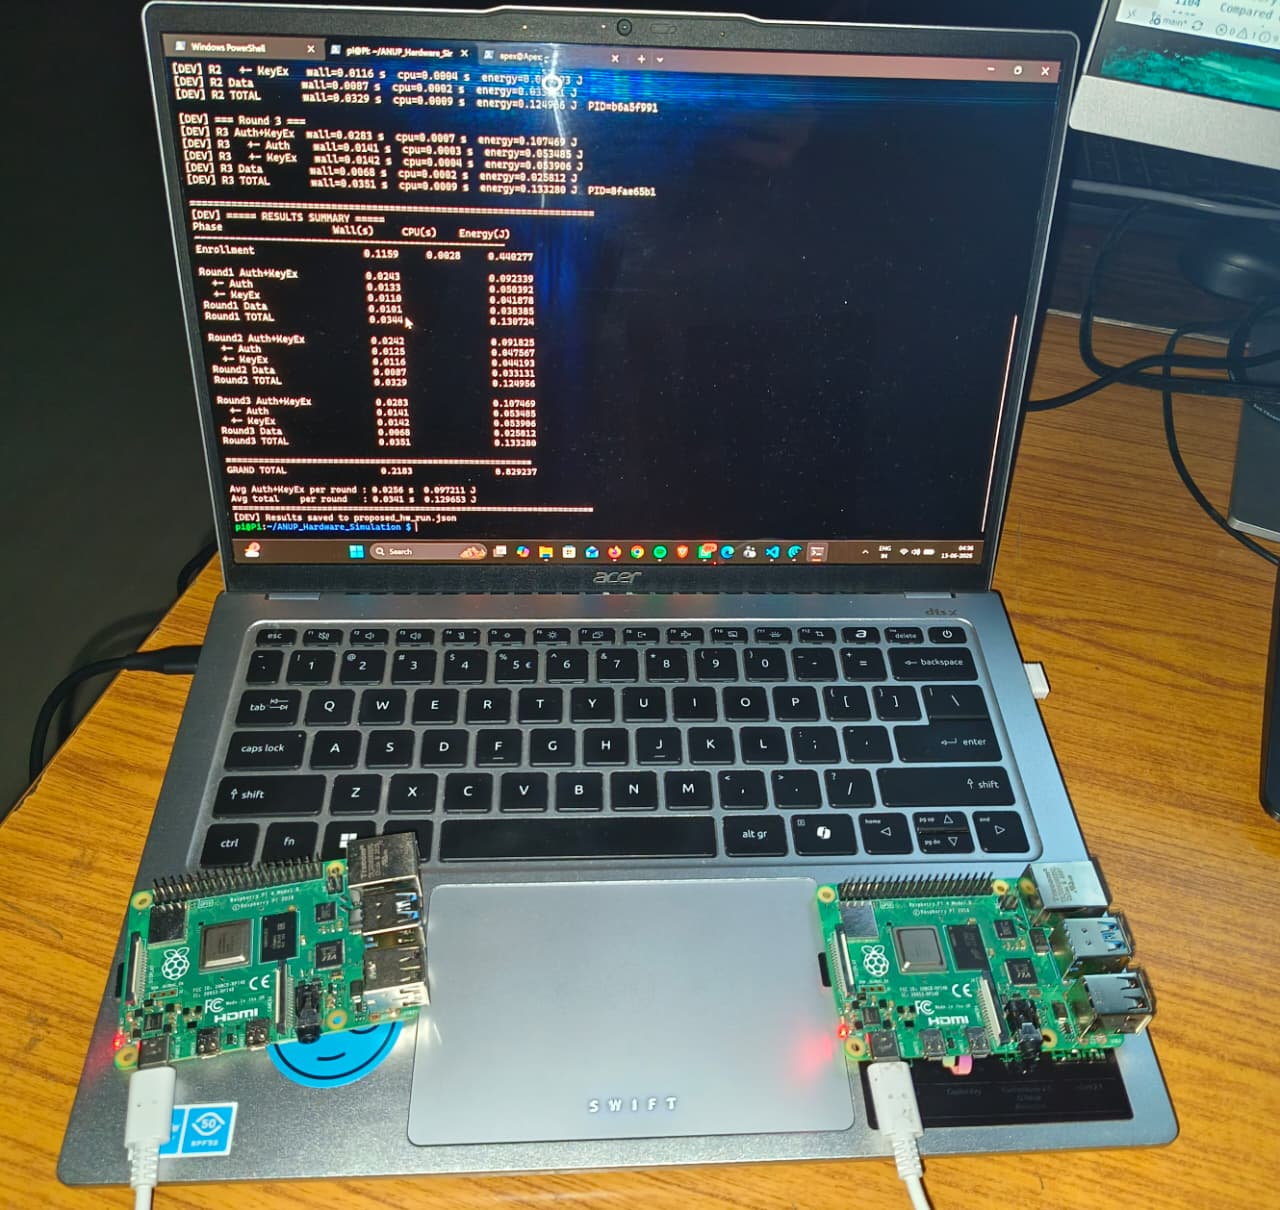
\includegraphics[width=0.8\textwidth,height=0.52\textwidth,keepaspectratio]{RPI_HW}
  \caption{Hardware testbed: two Raspberry Pi~4B boards (left: authentication
           server; right: device) connected to a Windows laptop (gateway).}
  \label{fig:hw_setup}
\end{figure}

As illustrated in Figure~\ref{fig:hw_comparison}(a), DAuth achieves the lowest
per-round energy of \textbf{0.152\,J}, as it performs no pseudonym operations.
The proposed scheme consumes \textbf{0.286\,J} per round, which is approximately
88\,\% more than DAuth due to the additional SHA-256 evaluations for pseudonym
rotation and dual-state verification.
Despite this overhead, the proposed scheme remains \textbf{14.2\,\%} and
\textbf{52.5\,\%} more energy-efficient than Zhou et al.\ (0.333\,J) and LAAKA
(0.602\,J), respectively, confirming that the anonymity guarantee is achieved at a
cost well within the range of existing non-anonymous schemes.

The CPU time results in Figure~\ref{fig:hw_comparison}(b) follow the same ordering:
DAuth (0.040\,s), Proposed (0.075\,s), Zhou et al.\ (0.088\,s), and LAAKA (0.159\,s).
The proposed scheme reduces CPU time by \textbf{14.8\,\%} and \textbf{52.8\,\%}
relative to Zhou et al.\ and LAAKA, respectively, while incurring an 87.5\,\%
overhead compared to DAuth, consistent with the energy results.
These reductions are consistent with the lightweight XOR-hash operations and
decoupled AS design of the proposed scheme, which translate directly to measurable
gains in physical energy and execution time on real hardware.

\begin{figure}[!ht]
  \centering
  
\includegraphics[width=0.95\textwidth]{fig_hw_comparison}
  \caption{Hardware-based performance: (a)~energy consumption and (b)~CPU time
           per authentication round on Raspberry Pi~4B
           (Proposed vs.\ DAuth vs.\ LAAKA vs.\ Zhou et al.).}
  \label{fig:hw_comparison}
\end{figure}

The inconsistency between hardware and simulation-based results arises due to the
disparity in scale, where a 100-node network is assumed in simulation whereas the
hardware setup involves only two Raspberry Pi platforms.
